%!TEX root = _thesis.tex
\chapter{序論}

\section{はじめに}
脳卒中麻痺リハビリテーションの目標は,食事,更衣,入浴などの日常生活動作ができるように患者の麻痺肢機能を改善することである.麻痺肢機能の改善を促進する介入方法の有効性を評価するためには,介入後の日常生活において,患者の麻痺肢使用量が実際に増えたか否かについて,リハビリテーションの効果を定量的に測る手法が必要である.しかしながら,病院やリハビリ施設で実施する検査では,質問紙やヒアリングによる調査が主体であり,日常生活における麻痺肢使用量を正確に評価することができない.さらに,診療所や研究所で行われるテストでは,日常生活上での患者の麻痺肢使用量を計測することができない.現在,日常生活上の麻痺肢使用量を測定する手法として,Accelerometryが一般的である.しかし,この手法は加速度センサを用いており,手指の使用量を正確に計測,評価することができない.そのため,本研究では日常生活において,麻痺患者の麻痺肢使用,特に,手指の使用量を計測,評価する手法を提案する.

\section{日常生活動作(Activities of Daily Living)}
日常生活動作(ADL)とは食事,更衣,入浴など,日常生活を営む上で必要となる動作のことである.麻痺患者の多くは,日常生活動作をするのに必要な,肢機能が健常者に比べ低い.
麻痺肢の使用が障害回復に効果がある\cite{Zeiler2017}.




\section{上肢機能評価結果を用いた臨床判断}
麻痺肢機能評価から導かれた結果は,臨床医が患者の麻痺肢機能を治療,回復させる計画を立てる際に,非常に重要である\cite{Lang2013}.加えて,臨床医が麻痺障害後の麻痺肢機能や,その障害の回復を予測する際,麻痺肢機能評価の結果を見て判断を行う.複数の疫学的なデータから麻痺の回復は,時間経過と関係があると示唆されており,最も障害の回復が見込めるのは,障害が引き起こってから三カ月以内であると言われている.麻痺の早期の障害の度合いは,最終的な運動障害に関係しており,軽度の障害である場合は,短期間で障害が回復し,3~6週間前後で障害が完治する.


\section{診療所や研究所で行われる上肢機能の評価手法}

\subsection*{Action Research Arm Test}
ARATは麻痺患者のために作成された,上肢機能の評価基準である\cite{}.

\subsection*{Box and Block Test}
Box and Block Test\cite{T.2005,Mathiowetz1985,Desrosiers1993,Lin2010}は実施が簡単かつ実施時間が短い上肢機能評価手法であり,ブロックの把持,移動,解放動作を評価する手法である.
被験者は,1分間で多くのブロックを箱から別の箱に移動させることを指示される.この手法では,上肢機能の能力を1分間に動かしたブロックの個数で評価する.
\begin{figure}[H]
  \centering
  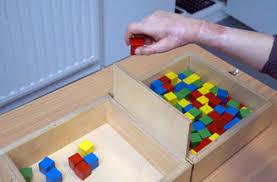
\includegraphics[width=0.8\linewidth]{fig/ch1/babt}
  \caption{Block and Block Test}
  \label{fig:babt}
\end{figure}



\subsection*{Nine-Hole Peg Test}
Nine-Hole Peg Testは手の器用さを測る簡単な手法である.被験者はペグをホールに刺し,刺した九つのペグを全て抜き取ることを指示される.テストの開始からペグを全て取り終えるまでの時間を計測し,その時間により,被験者の手の器用さを評価する.
\begin{figure}[H]
  \centering
  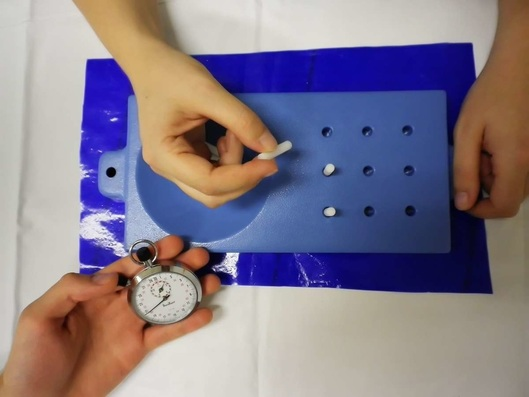
\includegraphics[width=0.8\linewidth]{fig/ch1/nhpt}
  \caption{Nine-Hole Peg Test}
  \label{fig:nhpt}
\end{figure}

\subsection*{Action Research Arm Test}
Action Research Arm Testは片側不全麻痺の患者の上肢機能評価手法である.この手法は19項目を握る,把持,ピンチ,全身運動の四つのサブスケールに
分け評価する手法である.上肢機能は各項目ごと0から3の四段階で評価され,各項目の評価が3であり,合計評価が57である場合,健常者と同等の上肢機能であると評価される.
\begin{figure}[H]
\begin{center}
\begin{tabular}{cc}
\subfigure[ARAT Kit]{
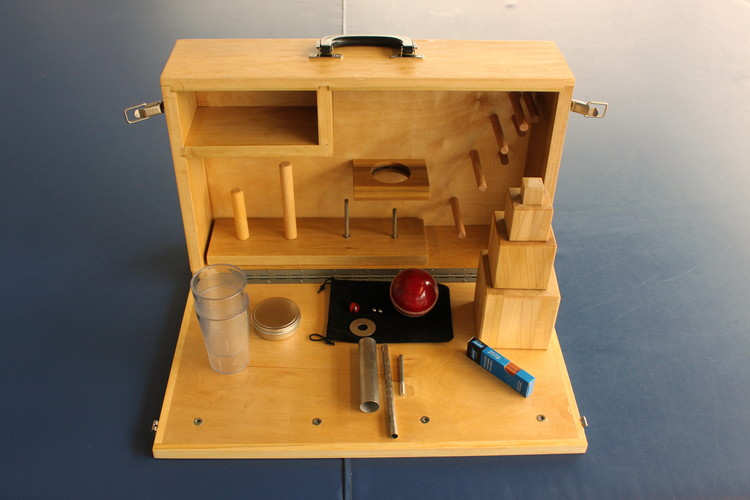
\includegraphics[scale=0.3]{fig/ch1/ARAT_kit}
} &
\subfigure[ARAT Score Sheet]{
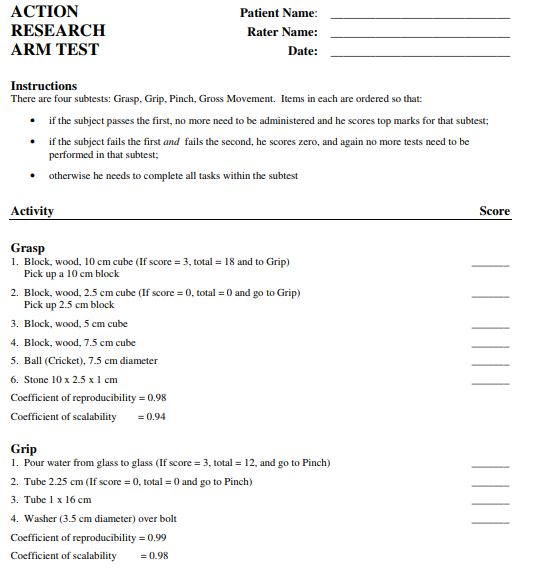
\includegraphics[scale=0.3]{fig/ch1/ARAT_SCORING}
} \\
\end{tabular}
\end{center}
   \caption{Action Research Arm Test}
\label{fig:ARAT}
\end{figure}


\subsection*{Motor Activity Log}

片上肢麻痺患者の日常生活上での麻痺肢使用量を測る標準的手法としてMotor Activity Log(MAL)\cite{Taub2006,Uswatte2005,Uswatte2000}がある.MALは,医師が患者に対し,麻痺肢使用の量と質について直接問う,質問形式の手法であり,測定結果が患者の認知レベルによる影響や質問者の主観的影響を受ける問題がある.そのため,客観的な測定手法が必要である.MALの質問項目は,一般的な日常生活動作に関する質問である.日常生活動作とは,電気のスイッチをオンにする動作や引き出しを開ける動作といった,日常生活を営む上で最低限必要な動作である.MALの評価用紙をFig.\ref{fig:Motor Activity Log}に示す.MALの質問項目は30項目あり,日常生活動作時の麻痺肢使用の量と質について11段階の評価で患者が答える.

\begin{figure}[H]
\begin{center}
\subfigure[Score sheet]{
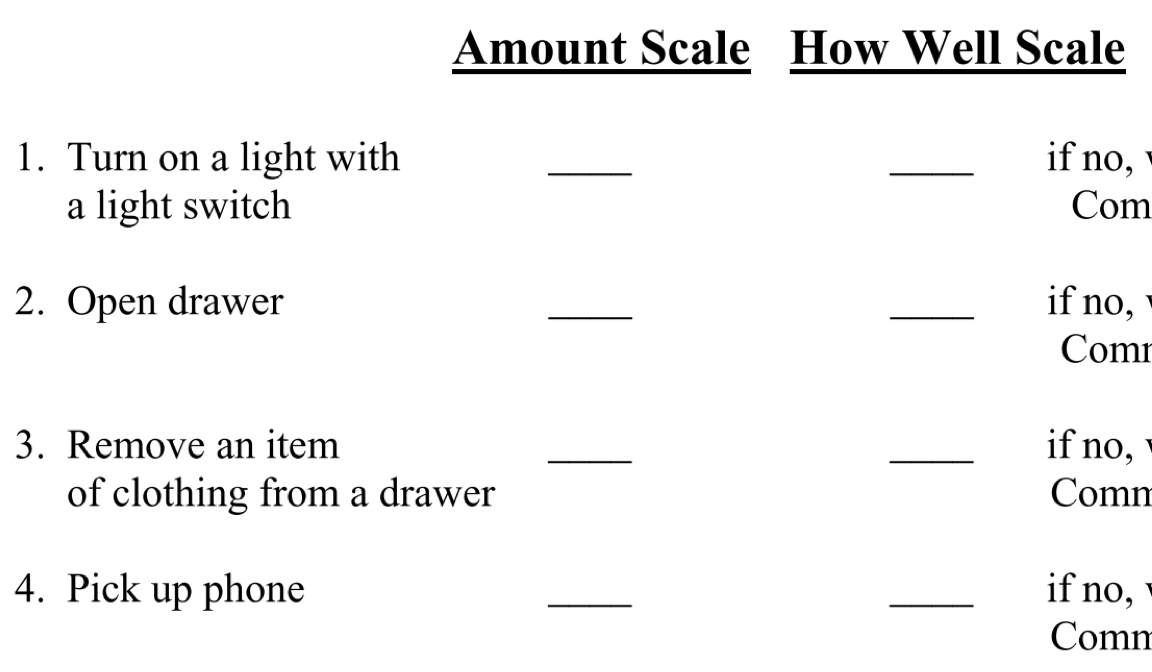
\includegraphics[scale=0.5]{fig/ch1/mal}
}
\begin{tabular}{cc}
\subfigure[Amout Scale]{
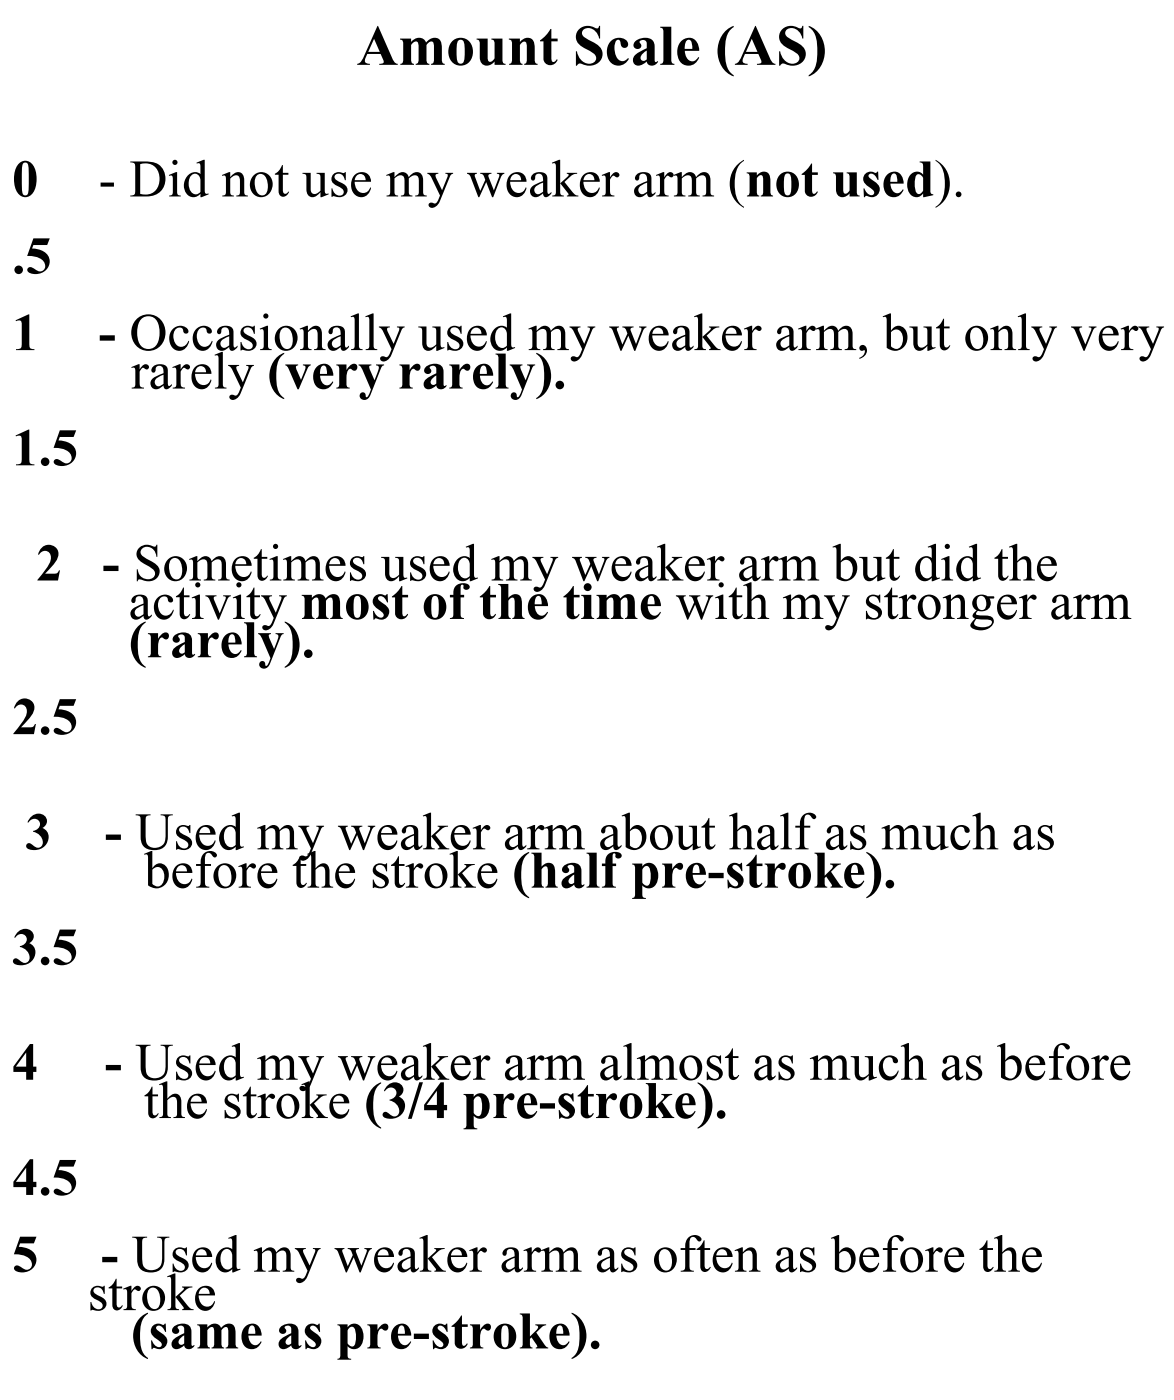
\includegraphics[scale=0.3]{fig/ch1/amount}
} &
\subfigure[How Well Scale]{
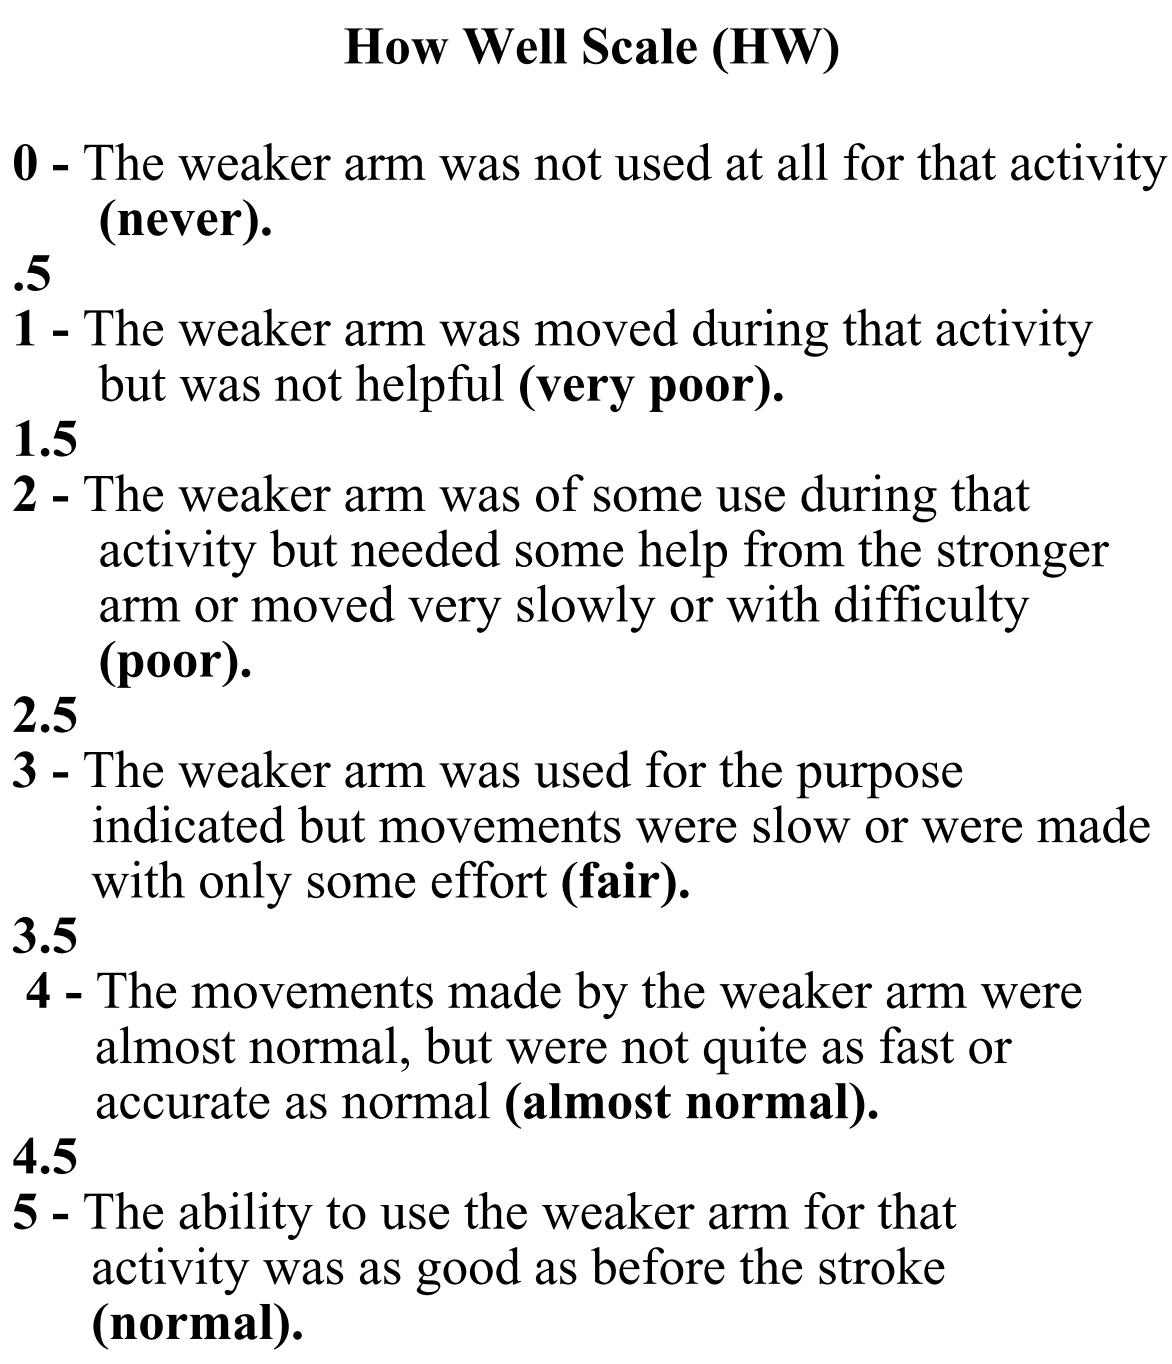
\includegraphics[scale=0.3]{fig/ch1/how}
} \\
\end{tabular}
\end{center}
   \caption{Motor Activity Log}
\label{fig:Motor Activity Log}
\end{figure}

これらの手法は,患者の運動機能を計測,評価することが可能である.

しかし,これらの手法は,定量的でない
また,日常生活上での患者の麻痺肢使用量を計測することができず,ADLが向上しているかの評価を行うことができない.



\section{定量的上肢使用量計測に関する研究}
\subsection*{Accelerometry}
Accelerometry\cite{Chen2005,Hayward2016,Dwiputra2017,VanDerPas2011,VanDerLee2004,Thrane2011}をFig.\ref{fig:Accelerometry}に示す.Accelerometryは,加速度計が埋め込まれた腕時計型のウェアラブルデバイスで上肢の使用量を測る手法である.Accelerometryは麻痺肢の手首に装着することで,麻痺肢の使用量を測定する.データ記録装置とバッテリーが内蔵されているため,麻痺肢使用量の常時計測に向いている\cite{VanDerPas2011}.しかし,この手法で計測される加速度データはノイズを多く含み,信頼性の高いデータを得ることができない.加速度データに混入するノイズは,測定された加速度が所定の時間内に,閾値を超える場合にのみ,麻痺肢使用のスコアを増加するといった手法の閾値フィルタを用いて低減することができる.このアプローチによって得られたスコアは日常生活において,腕を動かした時間と高い相関を持つことが示されている.しかし,閾値フィルタを使用したノイズ低減を行った場合,加速度が閾値に達しない小さな手の動きが見落とされる可能性がある.また,加速度計が手首に装着されているため,手首や手の精密な動きを計測できない問題がある.これらの理由から,Accelerometryは指の使用量の測定には向かない\cite{Uswatte2000}.
また,Accelerometryはタスクを行なっているのか,歩行時に手を振っているのかということを見分けられない.歩行時に腕を振っていることを検知する手法があるが,この手法は,足やつま先などに追加のAccelerometryを装着することを必要とする\cite{Ullery2015}.
さらに,Accelerometryはどのタスクをしているのかを見分けることも難しい\cite{Hayward2016}.
\begin{figure}[H]
  \centering
  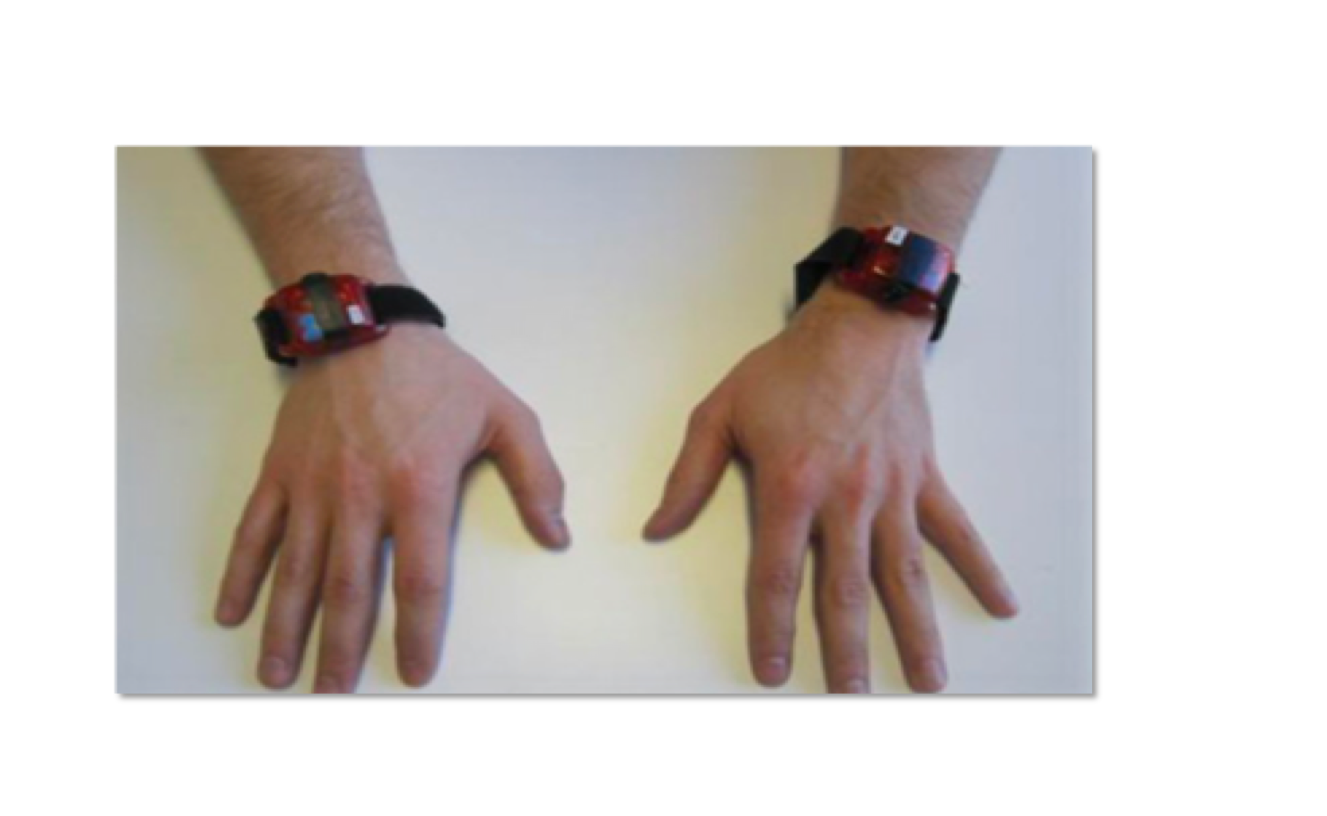
\includegraphics[width=0.8\linewidth]{fig/ch1/acc}
  \caption{Accelerometry}
  \label{fig:Accelerometry}
\end{figure}



\subsection*{Data Glove}
Data gloveは手袋型のセンシング機器である.手袋の中に,曲げセンサまたは光ファイバーが内蔵されている.Data gloveは手全体を覆うセンサが存在しているため,センサによる指や手の動きの阻害や,
Data gloveの取り外しによる煩雑さ,水で手を洗えないといった問題がある.

\begin{figure}[H]
  \centering
  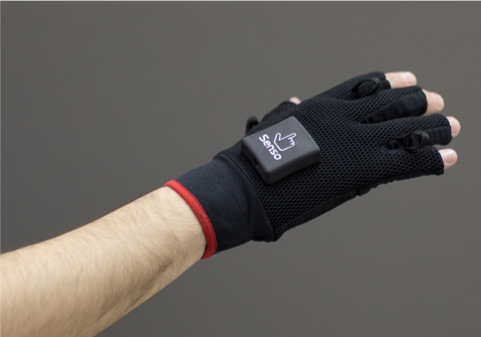
\includegraphics[width=0.6\linewidth]{fig/ch1/dataglove}
  \caption{Data glove}
  \label{fig:Data glove}
\end{figure}

\subsection*{Motion Capture System}
Motion capture systemはカメラ画像や赤外線距離センサによって,人体の動きをデジタルデータ取得するシステムである.手のモーショントラッキングに特化した,モーションキャプチャシステムにLeap Motionがある.Leap Motionは赤外線カメラにより,手の動きをトラッキングするシステムである.しかし,精度の問題から指の動きといった小さな動きを取得するのは難しい.また,モーションキャプチャシステムを構成する計測機器を常に持ち運んで運用することは難しい.そのため,常に持ち運びができ,精度よく指のトラッキングが行えるシステムが必要である.


\begin{figure}[H]
  \centering
  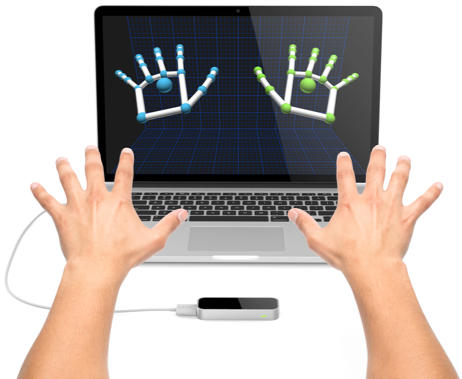
\includegraphics[width=0.6\linewidth]{fig/ch1/mcs}
  \caption{Motion Capture System(Leap Motion)}
  \label{fig:Motion Capture System}
\end{figure}


\subsection*{Manumeter}
Manumeter\cite{Friedman2014}は磁力計と磁石の指輪を用いて手首や指の使用量を測定する手法である.ManumeterをFig.\ref{fig:Manumeter}に示す.手首に取り付けてあるデバイスは磁力計,加速度計とデータ記録のためのストレージ,マイクロコンピュータで構成されている.指の動きを磁石と磁力計間の磁力変化により推定し,指の使用量を測定する.本手法は指の使用量の測定精度が低いという問題点がある.
\begin{figure}[H]
  \centering
  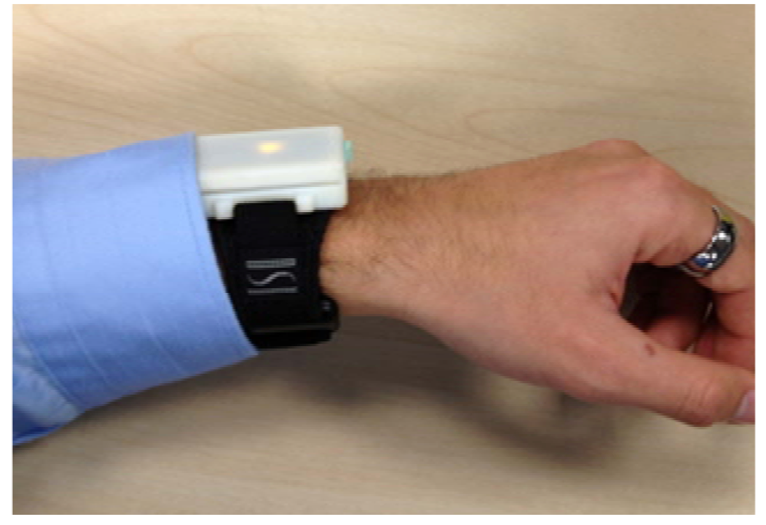
\includegraphics[width=0.6\linewidth]{fig/ch1/manumeter}
  \caption{Manumeter}
  \label{fig:Manumeter}
\end{figure}

\subsection*{Behind The Palm}
手の甲の皮膚の皺をパターン認識することによって,指ジェスチャを識別するBehind The Palm\cite{Recognition2017}といった手法が発表されている.ャリブレーションによるユーザーへの負担が大きい,ジェスチャの認識ができるが,精確な手の動作の動きの認識ができないという問題がある.
\begin{figure}[H]
  \centering
  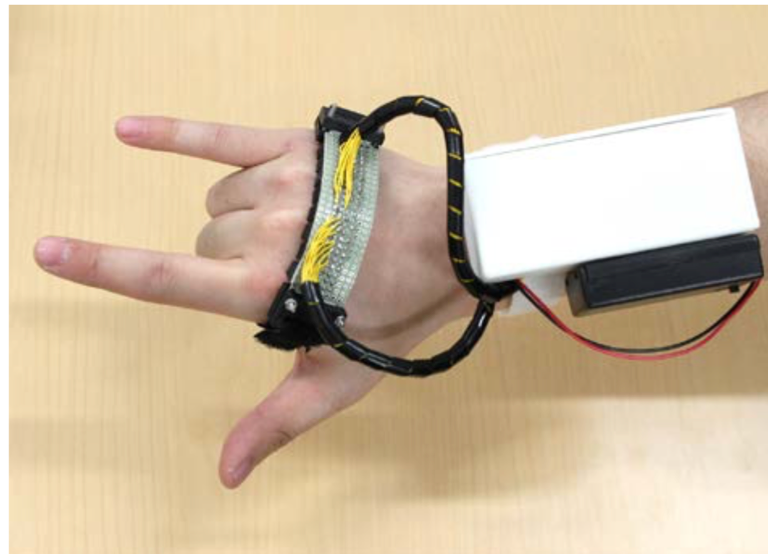
\includegraphics[width=0.6\linewidth]{fig/ch1/btp}
  \caption{Behind The Palm}
  \label{fig:Behind The Palm}
\end{figure}

研究レベルではData gloveやGoniometer,Motion capture system\cite{Binh2014,Valtin2017,Chen2003,Ren2011}などが手首や手の使用量を測定するために使用される.しかしながら,これらの手法は指の動きの阻害,空間的な制限といった問題があるため,日常生活における長時間の常時計測には向いていない.これらの理由から,依然として日常生活下の指の使用量を常時計測する手法は確立していない.本研究では,日常生活下の上肢片麻痺患者の麻痺肢使用,特に指の使用量を測る手法を提案し,手指使用量の常時測定のためのウェアラブルデバイスの開発を目的とする.


\section{本論文の構成}
本論文の構成を以下に記述する.第1章では本研究の背景と既存の研究について紹介する.第2章では,本研究で開発するデバイスの開発方法や,計測されたセンサデータの信号処理について記述する.第3章では,実験方法と結果を記述する.第4章では
実験によって得られた結果に対する考察と,本研究の課題を記述する.